\documentclass[a4paper]{article}

\usepackage[utf8]{inputenc}
\usepackage[ngerman]{babel}
\usepackage[T1]{fontenc}
\usepackage{listings}
\usepackage{hyperref}
\usepackage{graphicx}
\usepackage{gensymb}

\lstset{basicstyle=\ttfamily,columns=fullflexible}
\lstset{literate=%
	{Ö}{{\"O}}1
	{Ä}{{\"A}}1
	{Ü}{{\"U}}1
	{ß}{{\ss}}1
	{ü}{{\"u}}1
	{ä}{{\"a}}1
	{ö}{{\"o}}1
}
\newcommand*{\thead}[1]{\multicolumn{1}{c}{\bfseries #1}}

\begin{document}

\title{Heizungssteuerung}
\author{Viktor Saibel \& Daniel Tkocz}
\maketitle

\newpage

\tableofcontents

\newpage

\section{Einleitung}
%TODO bla
\section{Umsetzung}
\subsection{Grundlagen}
%TODO bla
Nach dem Herunterladen und Installieren der Software ETS5 von \href{https://www.knx.org/knx-de/software/ets/herunterladen/index.php}{knx.org} muss ein neues Projekt angelegt werden. Dies ist in Abbildung \ref{fig:1} zu sehen.

\begin{figure}[h!]
\centering
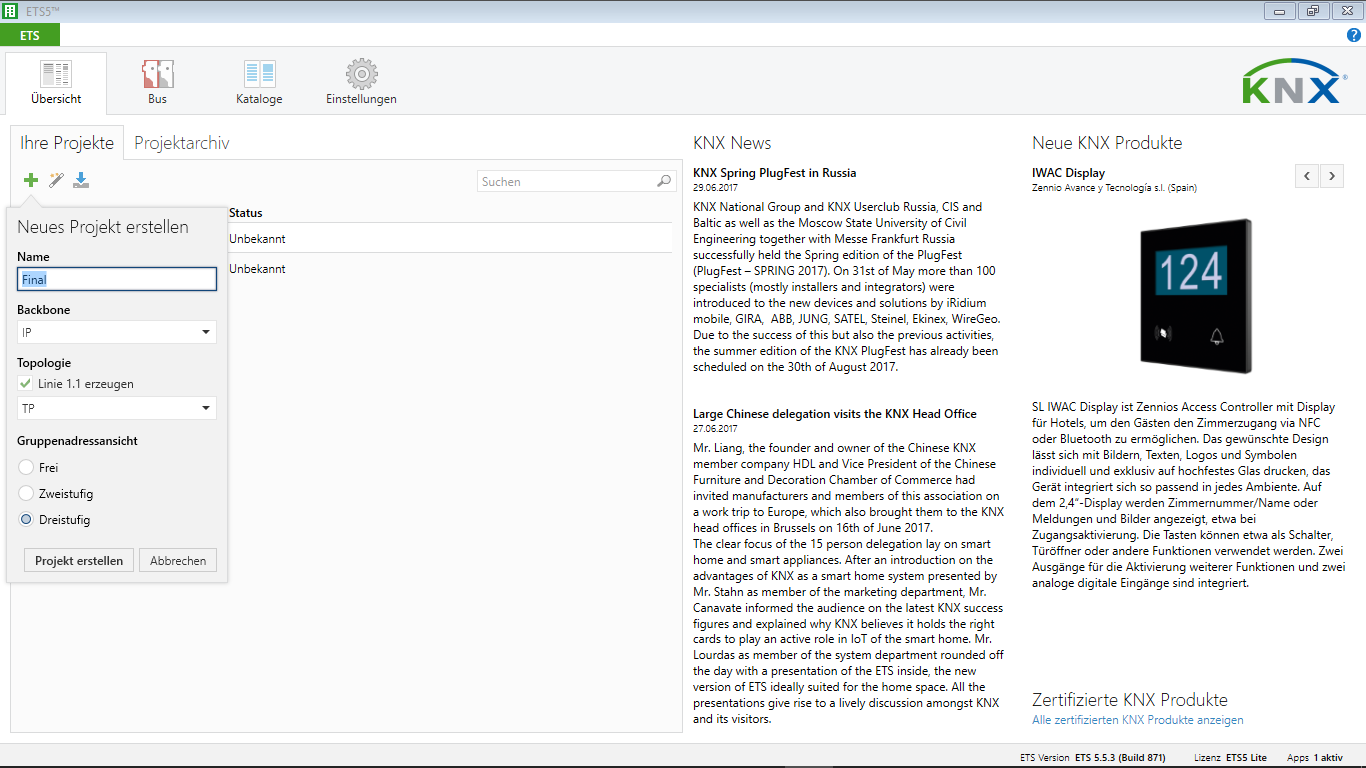
\includegraphics[width=13cm]{Doku/1}
\caption{Erstellen eines ETS5 Projekts}
\label{fig:1}
\end{figure}

Damit Komponenten zu dem Projekt hinzugefügt werden können, muss in dem Projekt ein Gebäude erstellt werden. In Abbildung \ref{fig:2} wurde Beispielhaft das C-Gebäude angelegt.

\begin{figure}[h!]
\centering
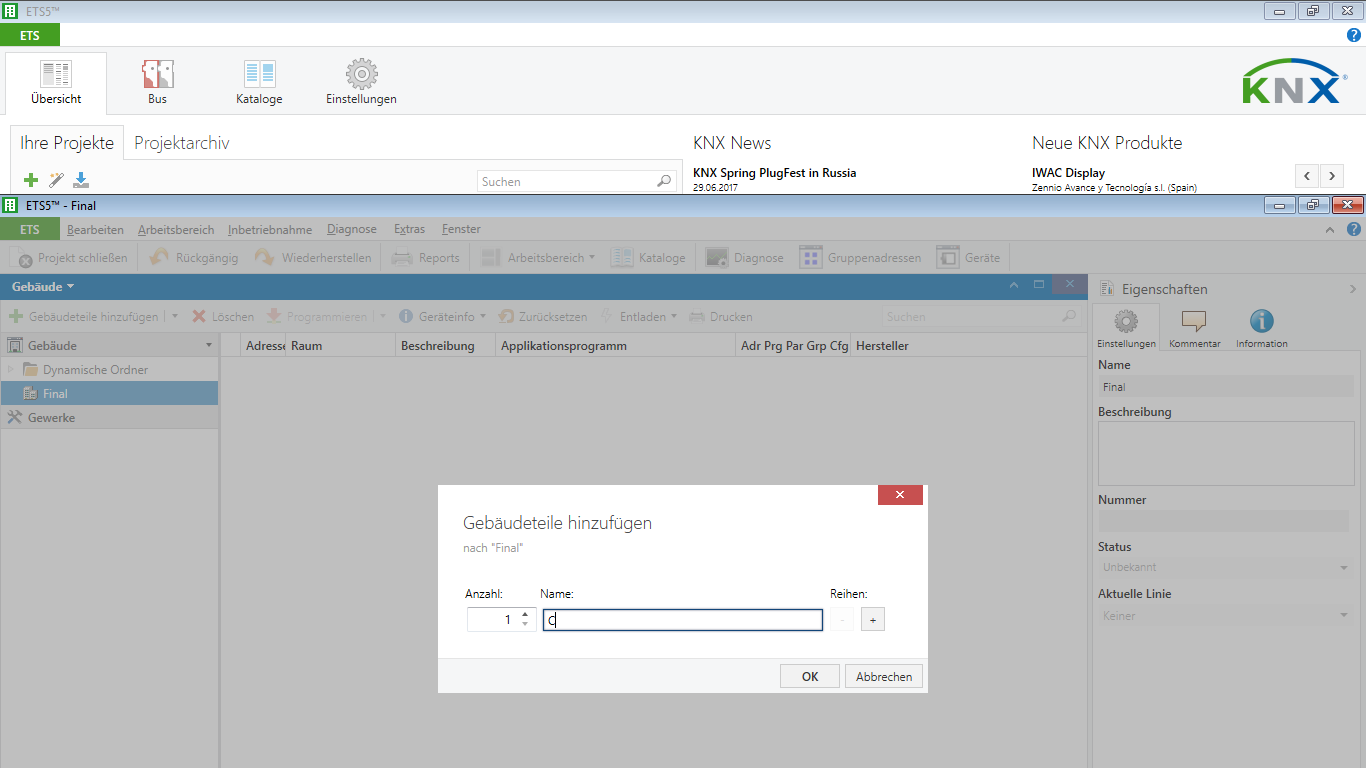
\includegraphics[width=13cm]{Doku/2}
\caption{Erstellen eines Gebäudes}
\label{fig:2}
\end{figure}

Ein Raum muss zusätzlich erstellt werden. Abbildung \ref{fig:3} zeigt wie Raum C031 angelegt wurde.

\begin{figure}[h!]
\centering
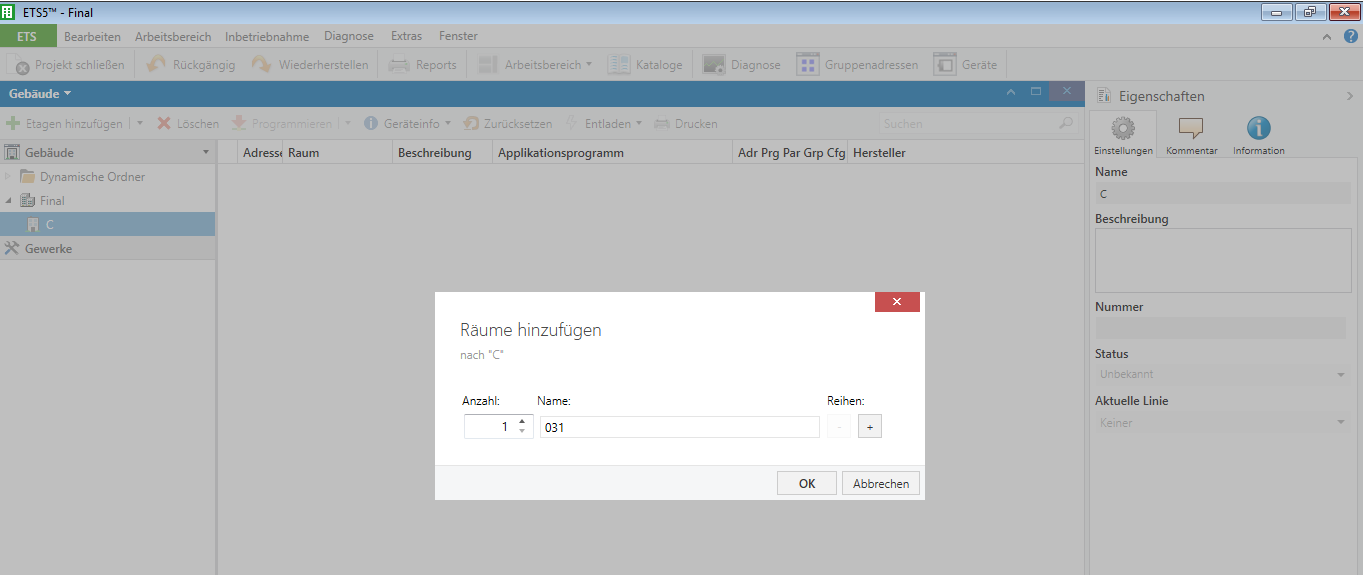
\includegraphics[width=13cm]{Doku/3}
\caption{Anlegen eines Raumes}
\label{fig:3}
\end{figure}

Sollen Geräte hinzugefügt werden, müssen von dem jeweiligen Hersteller die entsprechenden Konfigurationsdateien heruntergeldaen werden und in ETS5 importiert werden. Dazu werden Administrationsrechte benötigt. Abbildung \ref{fig:4} zeigt Beispielhaft eine Auswahl an möglichen Geräten.

\begin{figure}[h!]
	\centering
	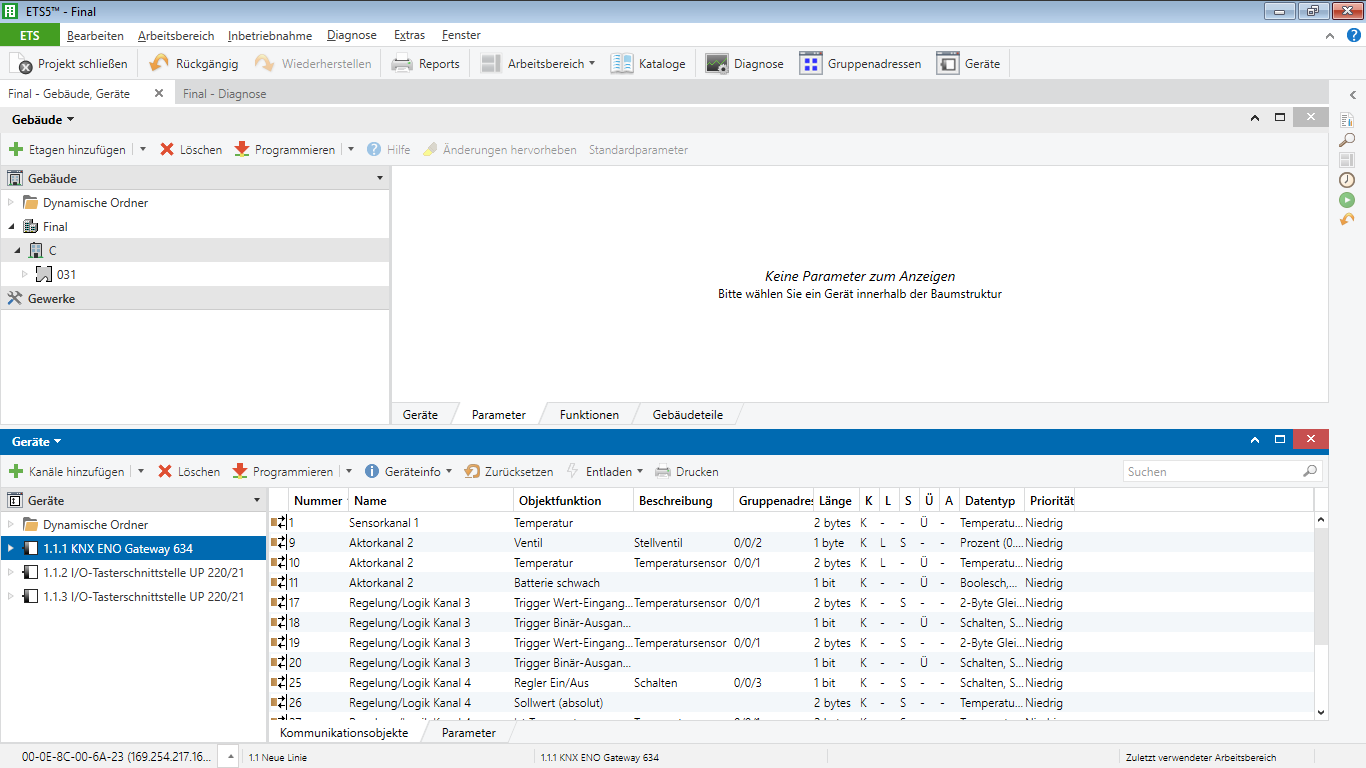
\includegraphics[width=13cm]{Doku/4}
	\caption{Übersicht der Gerätekonfigurationen}
	\label{fig:4}
\end{figure}

Per Drag \& Drop lassen sich diese Geräte in das Projekt importieren. Eine Auflistung aller Geräte des Projekts wird in Abbildung \ref{fig:5} gezeigt.

\begin{figure}[h!]
	\centering
	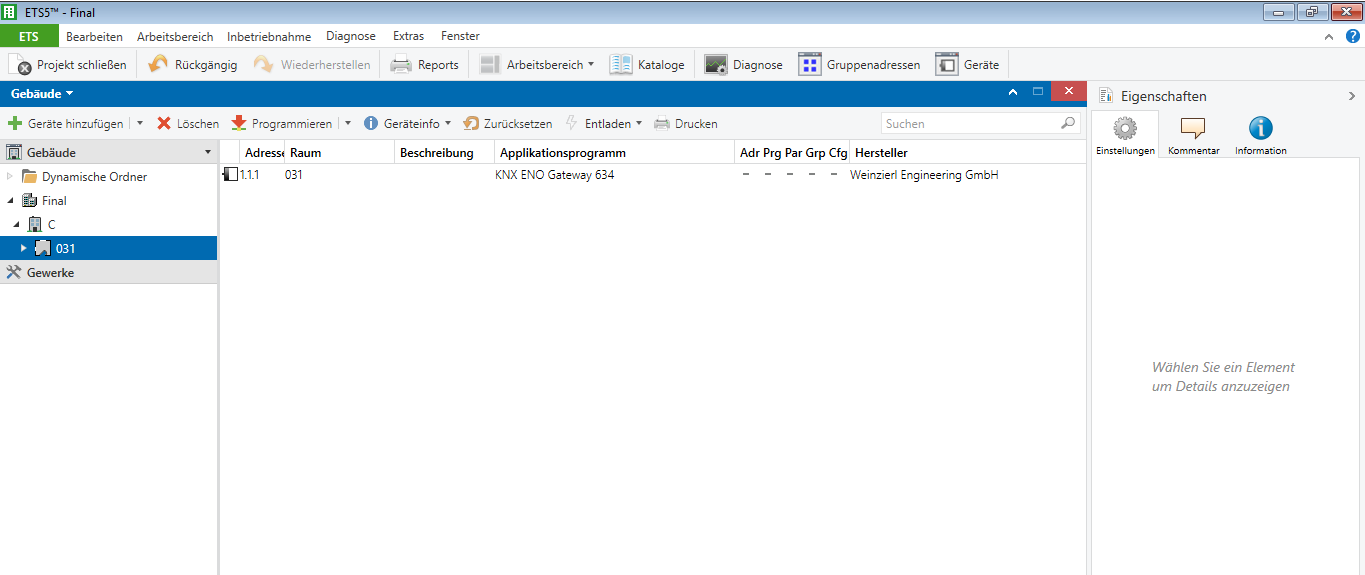
\includegraphics[width=13cm]{Doku/5}
	\caption{Übersicht der hinzugefügten Geräte}
	\label{fig:5}
\end{figure}

Damit die Geräte untereinander kommunizieren können müssen Gruppenadressen angelegt werden. Diese sind wie Geräte in einer dreistufigen Hierarchie angelegt. In den Abbildungen \ref{fig:6}, \ref{fig:7} und \ref{fig:8} kann betrachtet werden wie dies aussieht.

\begin{figure}[h!]
	\centering
	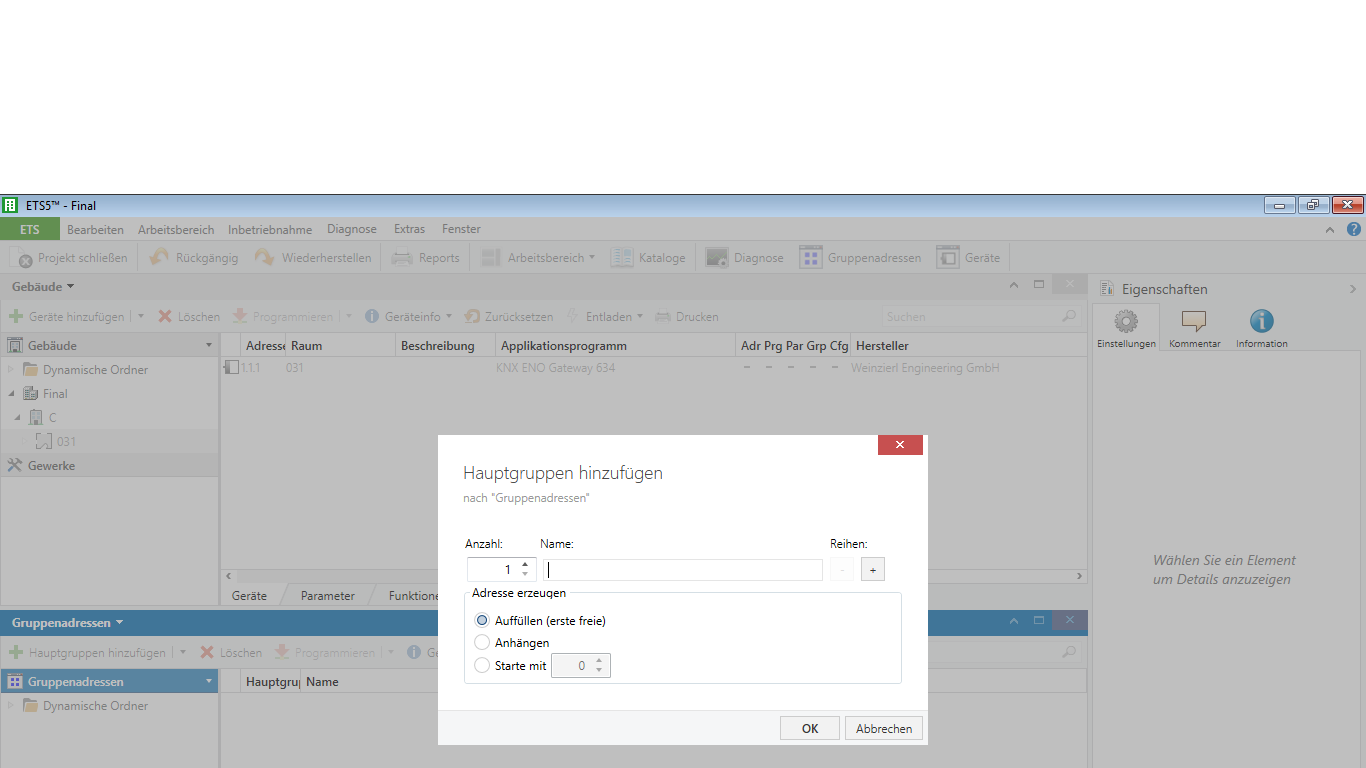
\includegraphics[width=13cm]{Doku/6}
	\caption{Anlegen einer Hauptgruppe}
	\label{fig:6}
\end{figure}

\begin{figure}[h!]
	\centering
	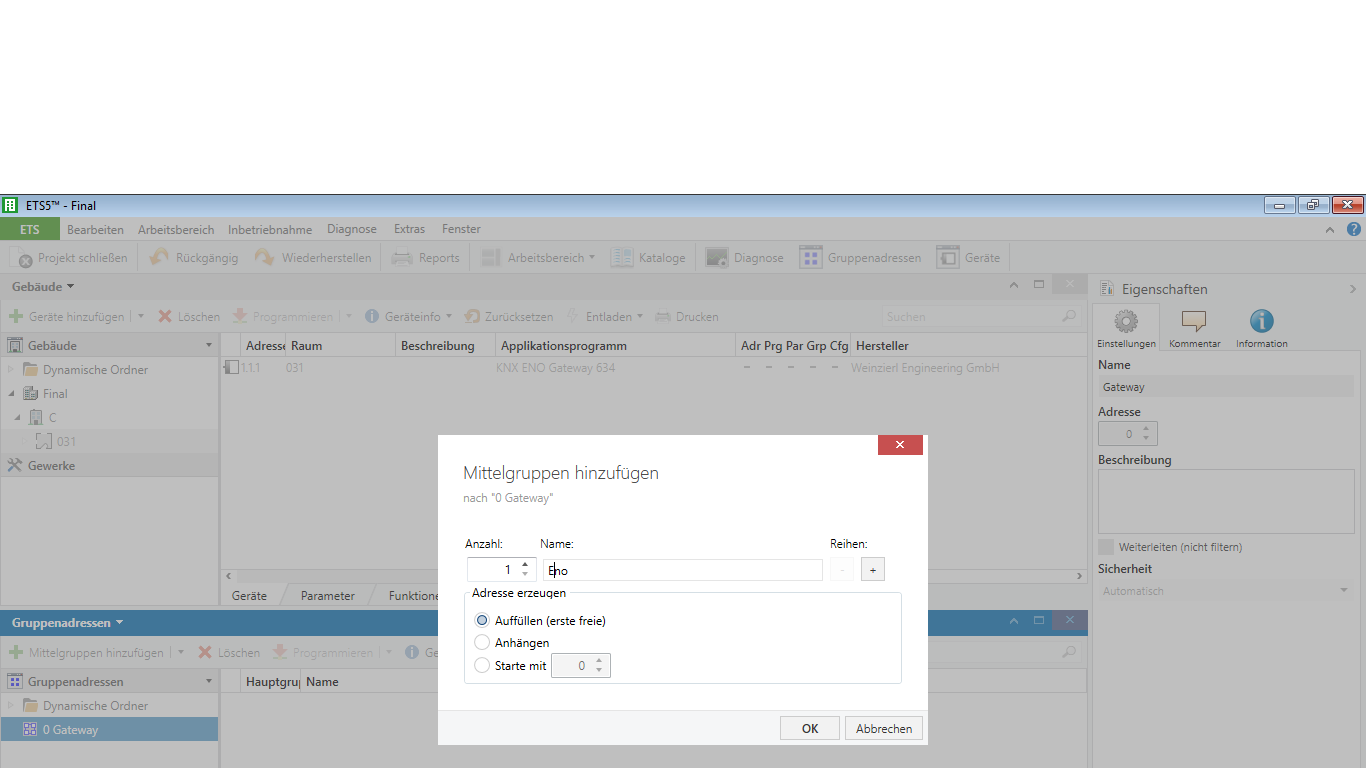
\includegraphics[width=13cm]{Doku/7}
	\caption{Erstellen einer Mittelgruppe}
	\label{fig:7}
\end{figure}

\begin{figure}[h!]
	\centering
	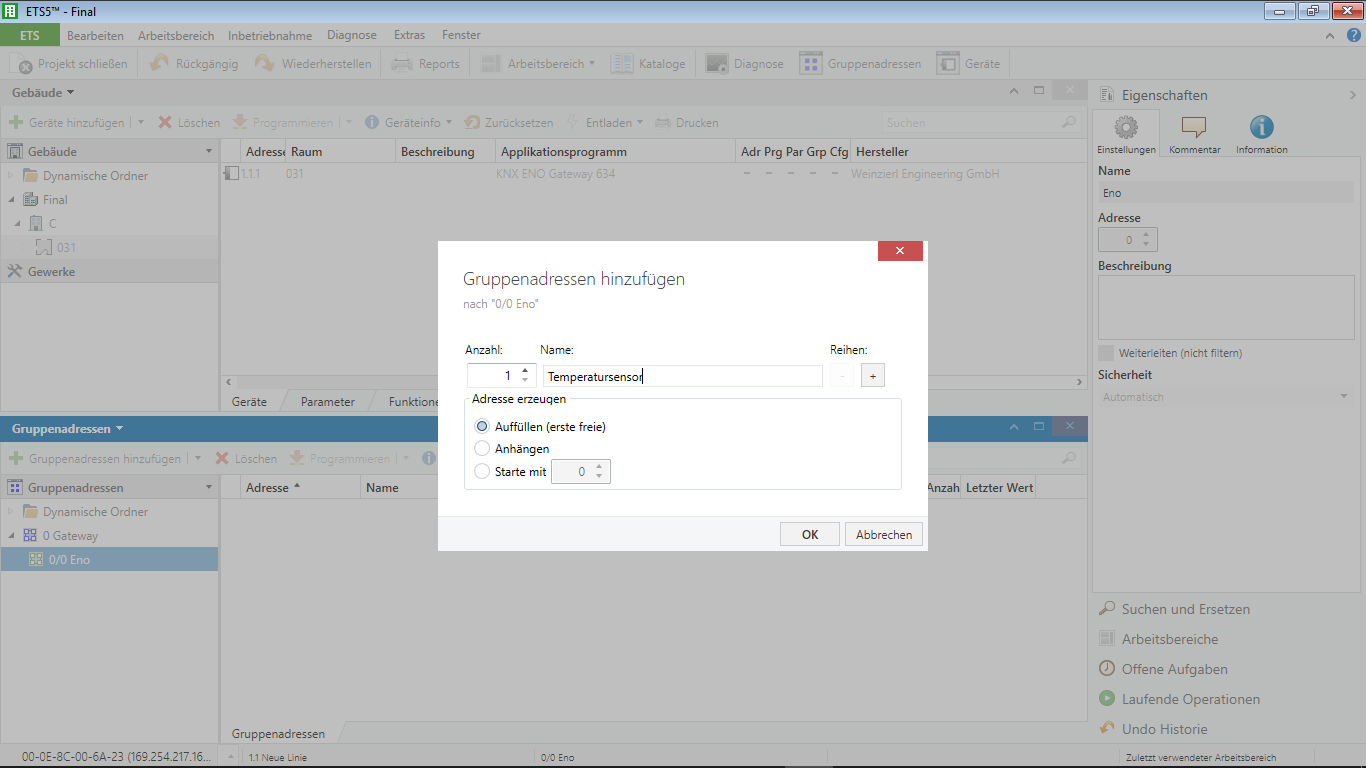
\includegraphics[width=13cm]{Doku/8}
	\caption{Gruppenadresse anlegen}
	\label{fig:8}
\end{figure}

\subsection{Konfiguration}

Als nächstes muss das Gerät konfiguriert werden. In diesem Fall wurde das KNX ENO Gateway 634 auf Kanal 2 als EnOcean Aktor mit Antrieb für Stellventil A5-20-01 definiert. Siehe dazu Abbildung \ref{fig:11}

\begin{figure}[h!]
	\centering
	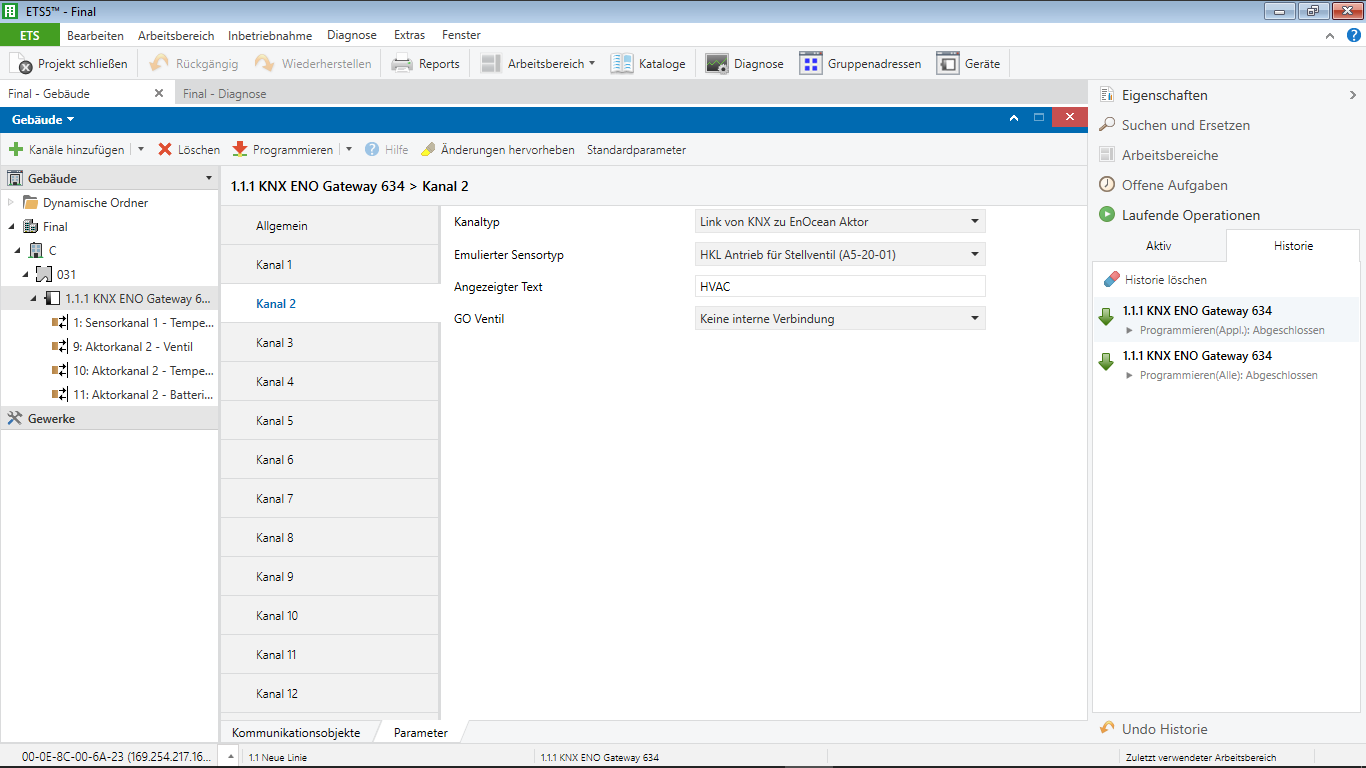
\includegraphics[width=13cm]{Doku/11}
	\caption{Konfiguration des KNX ENO Gateways}
	\label{fig:11}
\end{figure}

TODO TODO TODO Konfiguration des Gateways \& Thermostats TODO TODO TODO

Abbildung \ref{fig:12} zeigt die zyklische Temperaturmessung des Thermostats und übermittlung des gemessenen Wertes über EnOcean und KNX an den Busmonitor.

\begin{figure}[h!]
	\centering
	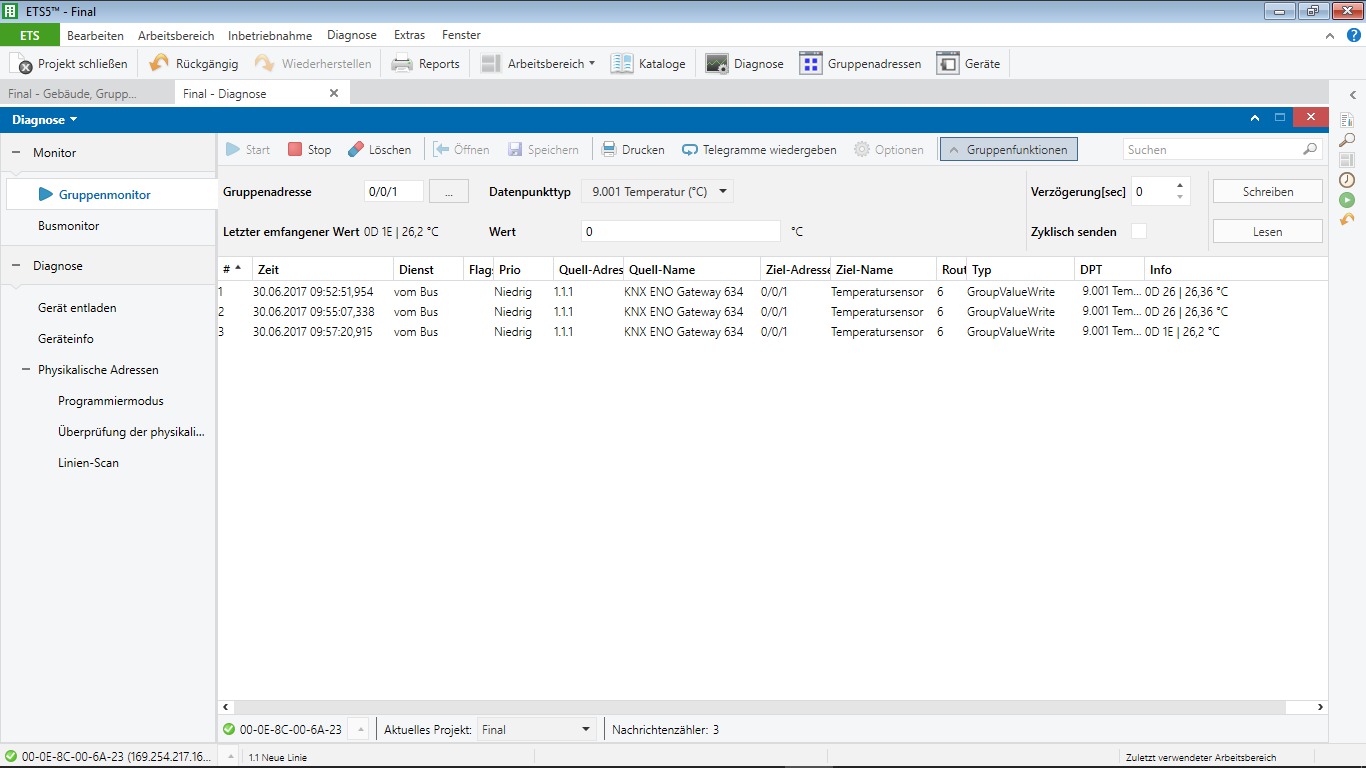
\includegraphics[width=13cm]{Doku/12}
	\caption{Konfiguration des KNX ENO Gateways}
	\label{fig:12}
\end{figure}

Es sei zu beachten, dass wenn man über den Busmonitor Werte Lesen und Schreiben möchte, die entsprechenden Berechtigungen gesetzt sein müssen. Wie in Abbildung \ref{fig:14} und \ref{fig:15} zu sehen ist, wurden dem Temperatursensor nur Leserechte gegeben während dem Ventil zusätzlich noch Schreibrechte gewährt wurden um den Wert manuell zu setzen.

\begin{figure}[h!]
	\centering
	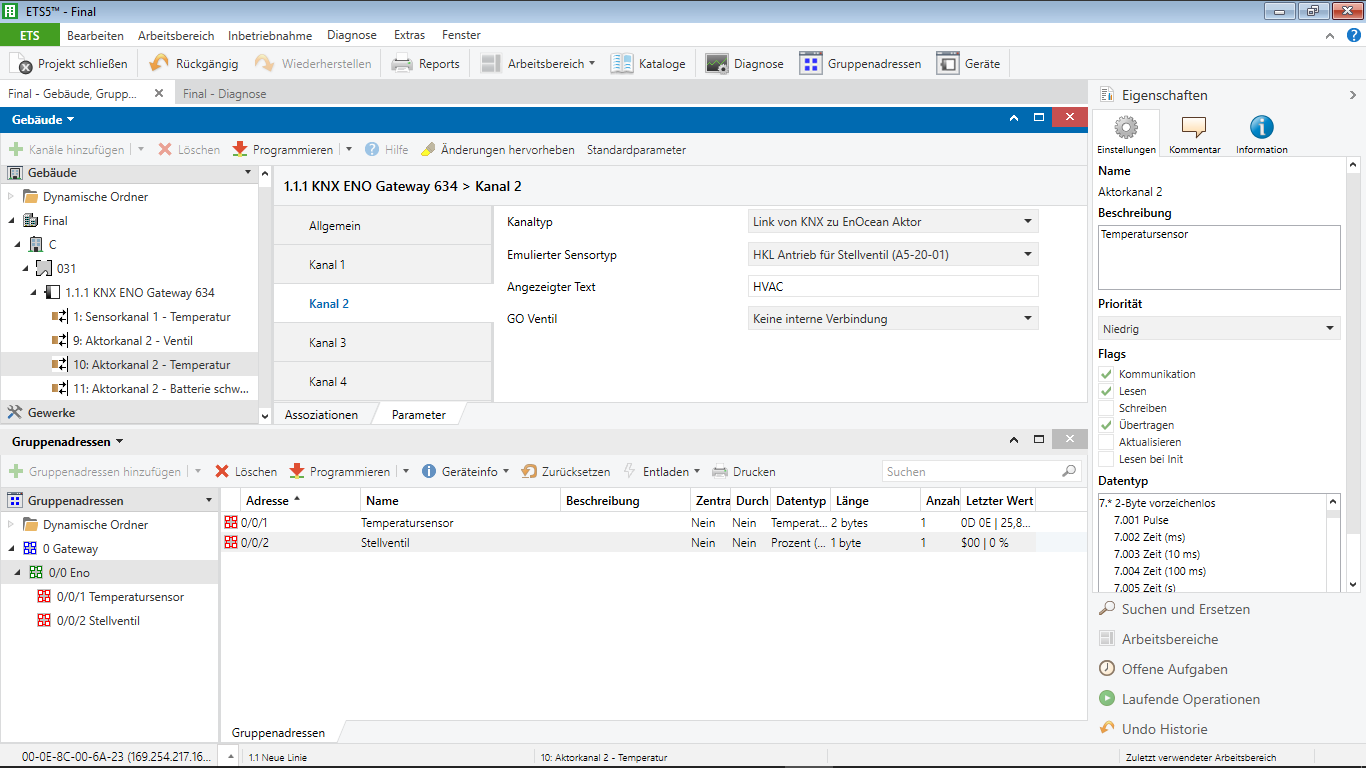
\includegraphics[width=13cm]{Doku/14}
	\caption{Rechte des Temperatursensors}
	\label{fig:14}
\end{figure}

\begin{figure}[h!]
	\centering
	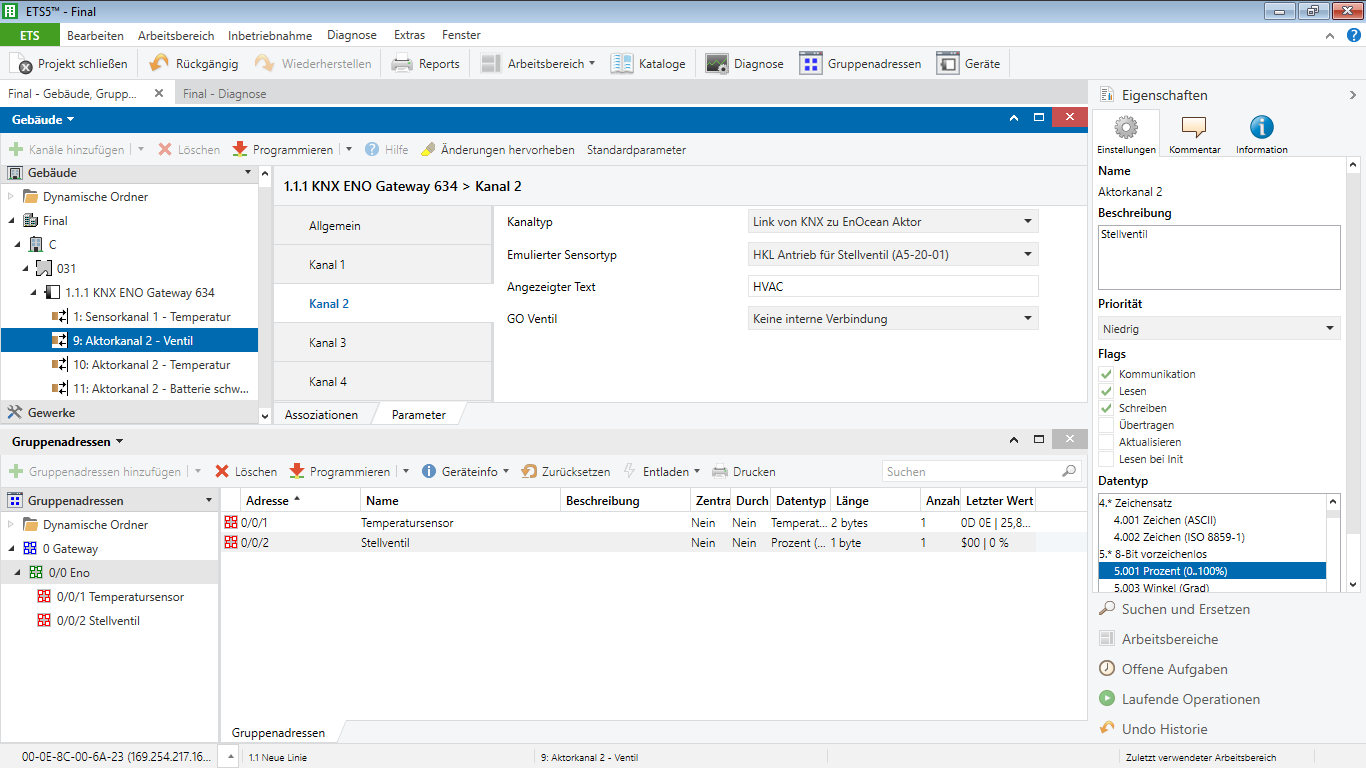
\includegraphics[width=13cm]{Doku/15}
	\caption{Rechte des Ventils}
	\label{fig:15}
\end{figure}

TODO Kanal4
Um das Thermostat in einem Regelbetrieb automatisch zu betreiben wurde eine Regel angegeben um die Temperatur zu regeln. Wie in Abbildung \ref{fig:16} zu sehen ist, wurde der Sollwert der Temperatur zu Testzwecken auf warme 30 $^{\circ}$C gesetzt.

\begin{figure}[h!]
	\centering
	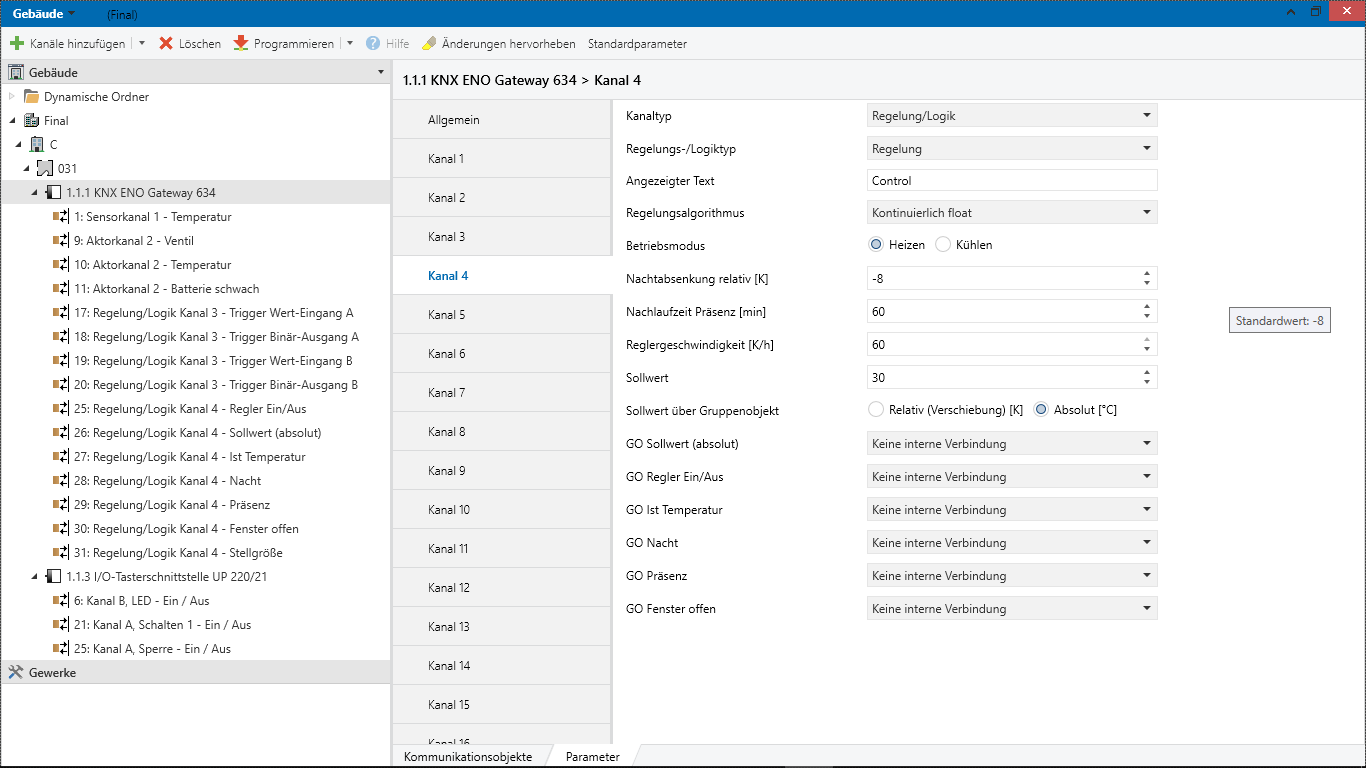
\includegraphics[width=13cm]{Doku/16}
	\caption{Regel zur Temperatursteuerung}
	\label{fig:16}
\end{figure}

Wie zuvor bereits erwähnt müssen die einzelnen Komponenten über Gruppenadressen miteinander verbunden sein um miteinander kommunizieren zu können.
Eine Übersicht über alle Gruppenadressen und deren Verknüpfung mit den jeweiligen Komponenten ist in den Abbildungen \ref{fig:17}, \ref{fig:18} und \ref{fig:19} zu finden.

\begin{figure}[h!]
	\centering
	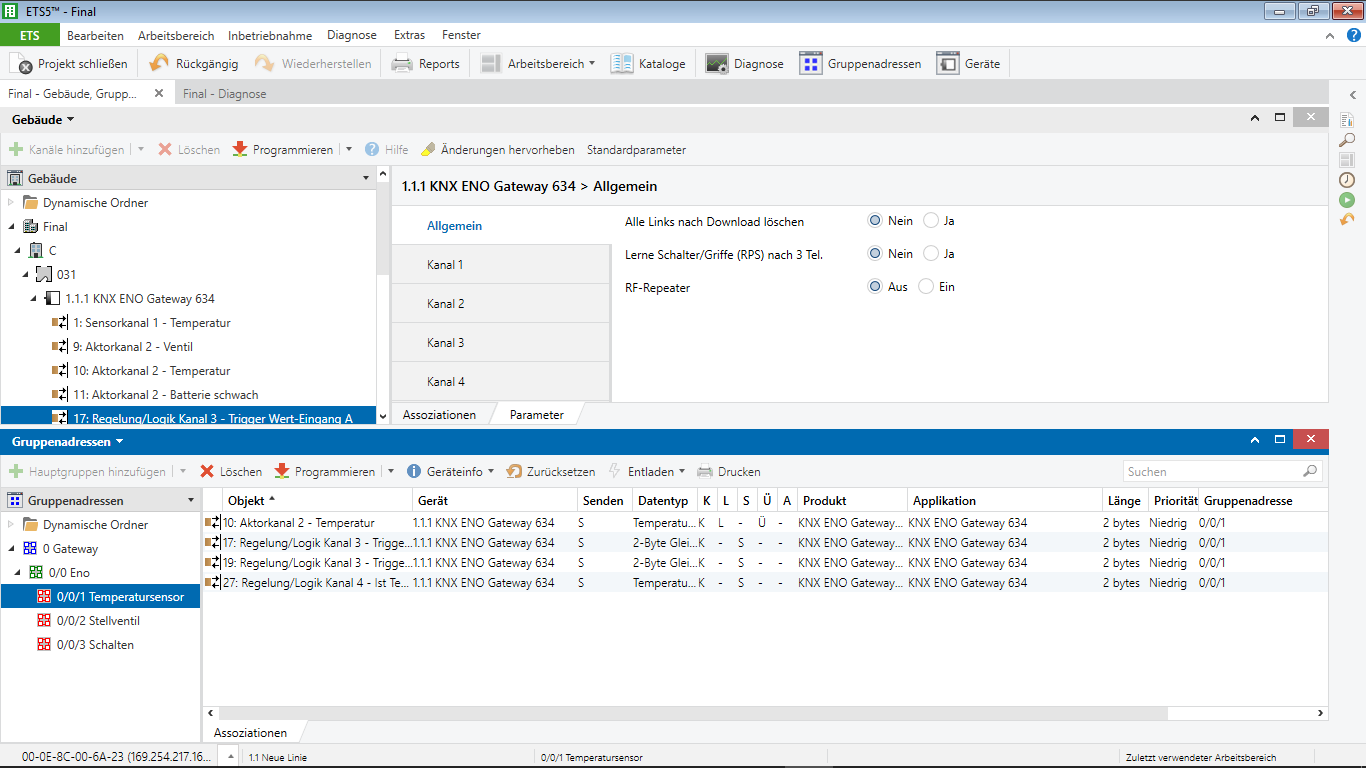
\includegraphics[width=13cm]{Doku/17}
	\caption{Gruppenadresse des Temperatursensors}
	\label{fig:17}
\end{figure}

\begin{figure}[h!]
	\centering
	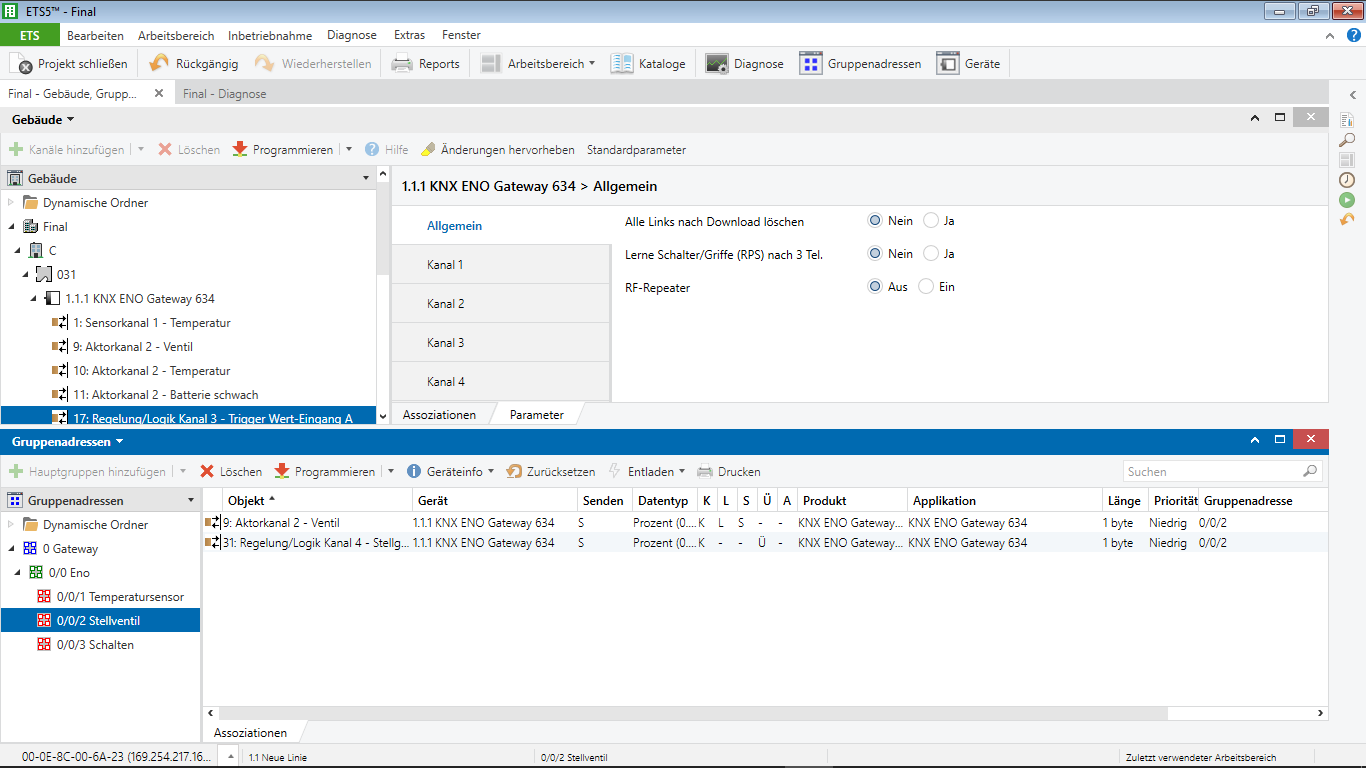
\includegraphics[width=13cm]{Doku/18}
	\caption{Gruppenadresse des Stellventils}
	\label{fig:18}
\end{figure}

TODO Taster textuell einführen.

\begin{figure}[h!]
	\centering
	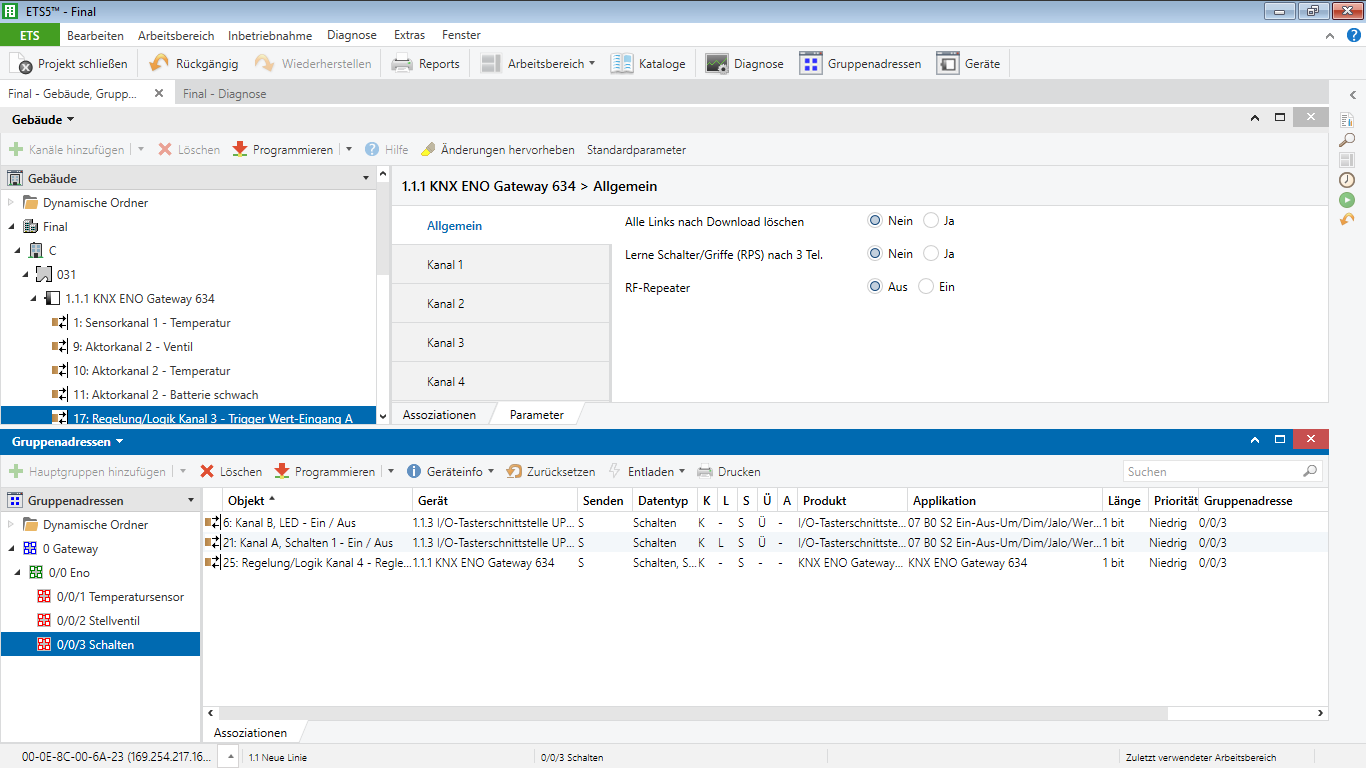
\includegraphics[width=13cm]{Doku/19}
	\caption{Gruppenadresse des Tasters}
	\label{fig:19}
\end{figure}

\begin{table}[h!]
\centering
\begin{tabular}{|l|l|}
\thead{Klassifizierverfahren} & \thead{Gewichtung}\\\hline
Token & 1,0\\\hline
Grammatik & 0,1\\\hline
Länge & 0,45\\\hline
\end{tabular}
\caption{Gewichtung}
\label{tab:weights}
\end{table}
\section{Fazit}
TODO FEHLER beschreiben (EnOcean)
Doku kacke
wartezeit 2min
google=nix
GO was ist das?
%TODO bla

\end{document}